\scanpage{1}
% not manuscript: couverture de l'Université de Montpellier / IMAG, « La "Longue Marche" à travers la théorie de Galois », cote n° 140-1, 36 pages.

\scanpage{2}
% S002-E01: upper right heading.
\margin{\uline{``Longue Marche''}}
% S002-E02: upper left, cancelled beginning and equation.
\[
\deleted{\underline{u}\unsure{\Rightarrow|=}}\unsure{\,\cdot\,|\,;\,}
\qquad \alpha=\underline{u}a^{-1}
\]
% S002-E03: detached expression under the heading.
\[
-\unsure{v|\nu}d^2+wcd+c^2
\]
% S002-E04: upper left.
\[
\underline{u}=\alpha\underline{a}
\]
% S002-E05: upper right.
\[
\det\bigl(d\rho+\unsure{c}\bigr)
=d^2\det\rho+cd\,\uline{\operatorname{Tr}\rho}+c^2
\]
% S002-E06: upper left matrix, without a label in the original.
\[
\begin{pmatrix}a&b\\c&d\end{pmatrix}
\]
% S002-E07: upper right matrix.
\[
\rho=\begin{pmatrix}0&\unsure{v_1|\nu_1}\\\unsure{v|\nu}&w\end{pmatrix}
\]
% S002-E08: left.
\[
a=\alpha^{-1}u
\]
% S002-E09: right.
\[
d_0\rho+c_0=
\begin{pmatrix}
c_0&d_0\unsure{v_1|\nu_1}\\
d_0\unsure{v|\nu}&d_0w+c_0
\end{pmatrix}
\]
% S002-E10: middle. The final matrix is left unfinished in the scan.
\[
\begin{pmatrix}a&b\\c&d\end{pmatrix}
\begin{pmatrix}c&d\\d\unsure{v|\nu}&dw+c\end{pmatrix}
=\left(\begin{array}{cc}ac+bd\unsure{v|\nu}&\\&\end{array}\right.
\]
% S002-E11: middle, overwritten top entries in the second factor.
\[
\underline{a}=\alpha^{-1}u
=\frac{1}{\delta_\alpha}
\begin{pmatrix}d&-b\\-c&a\end{pmatrix}
\begin{pmatrix}
\deleted{\unsure{A|B}}\inserted{\unsure{\mu}}&
\deleted{\unsure{B}}\inserted{\unsure{\lambda}}\\
0&1
\end{pmatrix}
\]
% S002-E12: continuation across the fold.
\[
=\frac{1}{\delta_\alpha}
\begin{pmatrix}
\deleted{\unsure{d|\delta}}\inserted{d}\mu&d\lambda-b\\
-c\mu&-c\lambda+a
\end{pmatrix}
=d_0\rho+\unsure{c_0|d_0}
\]
% S002-E13: lower middle.
\[
c_0=d\mu\unsure{/|\ne}\delta_\alpha
=\frac{-d\unsure{v|\nu}}{-\unsure{v^2|\nu^2}+wcd+\unsure{c^2}}
\]
% S002-E14: cancelled line; no closing parenthesis is written.
\[
\deleted{
d_0=\frac{1}{\delta_\alpha}(d\lambda-b)
=\frac{1}{\delta_\alpha}
\left(-\unsure{v|\nu}bd^2+\unsure{v_1|\nu_1}acd+w bcd\right.
}
\]
% S002-E15: immediately below the cancellation.
\[
d_0\unsure{v|\nu}=\frac{-c\mu}{\delta_\alpha}
\]
% S002-E16: abandoned beginning at left.
\[
d_0=-
\]
% S002-E17: lower right.
\[
c_0=\frac{d\mu}{\delta_\alpha}
\]
% S002-E18: lower right.
\[
d_0=\frac{-c\mu}{\delta_\alpha\unsure{v|\nu}}
\]
% S002-E19: cancelled calculation to the left of the box.
\[
\deleted{\det\underline{a}=\det\unsure{\,\cdot\,}}
\qquad
\deleted{\frac{\unsure{u|\mu}}{\unsure{\delta_\alpha|\delta}}}
\]
% S002-E20: cancelled mark beside the box.
\margin{\(\deleted{\unsure{\underline{a}}}\)}
% S002-E21: boxed expression, including the ambiguous sign after the parenthesis.
\[
\boxed{\underline{a}=\frac{\mu}{\delta_\alpha}
\left(\unsure{-|=}\frac{c}{\unsure{v|\nu}}\rho+d\right)}
\]
% S002-E22: lower left; the question mark is written above the equals sign.
\[
\det a\overset{?}{=}\delta_\alpha^{-1}\mu
\]
% S002-E23: bottom right. The terminal dots are present in the scan.
\[
\det\underline{a}=\left(\frac{\mu}{\delta_\alpha}\right)^2
\left[\frac{c^2}{\unsure{v^2|\nu^2}}
\bigl(-\unsure{vv_1|\nu\nu_1}\bigr)
\unsure{-|+}\frac{dc}{\unsure{v|\nu}}w+d^2\right]\ldots
\]
% S002-E24: lower-left pencil foliation.
\margin{1}

\scanpage{3}
% not manuscript: circulaire dactylographiée de l'Université des Sciences et Techniques du Languedoc, 18 septembre 1978, « Rentrée universitaire 1978-1979 », adressée au professeur Grothendieck; feuille à l'envers dans le scan.

\scanpage{4}
\mspage{1}

\[
\unsure{\widetilde{\Pi}_n^{\circ D}|\widetilde{\Pi}_n^D}
\unsure{\simeq|=}
\deleted{\unsure{\{}}
\{\tilde\rho,\tilde\sigma\mid\tilde\rho^n=\tilde\sigma^2\}
\qquad
\boxed{\tilde\rho^n=\tilde\sigma^2=\tilde\omega_0}
\quad\text{\unsure{élément} central}
\]

\diagram{\begin{tikzcd}[ampersand replacement=\&,column sep=small]
1\arrow[r]\&\mathbb Z\arrow[r]\&
\unsure{\widetilde{\Pi}_n^{\circ D}|\widetilde{\Pi}_n^D}\arrow[r,no head]\&
\Pi_n^D\arrow[r,no head]\&1
\end{tikzcd}}
ext. central

Posons
\[
\begin{aligned}
\boxed{\tilde\rho_0=\tilde\sigma\tilde\rho\tilde\sigma^{-1}\tilde\rho}
&=\tilde\sigma(\tilde\rho)\tilde\rho\\
&=(\tilde\sigma\tilde\rho)^2\tilde\omega_0^{-1}
\end{aligned}
\qquad
\boxed{\tilde\rho_i=\tilde\rho^{\unsure{i}}(\tilde\rho_0)}
\]
\margin{\deleted{$\unsure{+}$} $\tilde\rho_i$ relève $\rho_i$}

On a
\[
\begin{aligned}
\tilde\rho_{n-1}\tilde\rho_{n-2}\cdots\tilde\rho_0
&=\underbrace{\tilde\rho^{n-1}\tilde\rho_0\tilde\rho^{-(n-1)}}
\underbrace{\tilde\rho^{n-2}\tilde\rho_0\tilde\rho^{-(n-2)}}
\cdots(\tilde\rho\tilde\rho_0\tilde\rho^{-1})\tilde\rho_0\\
&=\tilde\rho^{n-1}\tilde\rho_0\tilde\rho^{-1}\tilde\rho_0\tilde\rho^{-1}
\cdots\tilde\rho^{-1}\deleted{\unsure{{}_0}}\tilde\rho_0\tilde\rho^{-1}\tilde\rho_0
\qquad\begin{gathered}(n\ \text{\unsure{facteurs}}\\\tilde\rho_0\end{gathered}\\
&=\tilde\rho^n\underbrace{(\tilde\rho^{-1}\tilde\rho_0)\cdots(\tilde\rho^{-1}\tilde\rho_0)}_{n\ \text{facteurs}}
=\underbrace{\tilde\rho^n}_{\tilde\omega_0}(\tilde\rho^{-1}\tilde\rho_0)^n
\end{aligned}
\]

or
\[
\tilde\rho^{-1}\tilde\rho_0
=\tilde\rho^{-1}\tilde\sigma\tilde\rho\tilde\sigma^{-1}\tilde\rho
=(\tilde\rho^{-1}\tilde\sigma)(\tilde\rho)
\]
. \unsure{donc}
\[
(\tilde\rho^{-1}\tilde\rho_0)^n
=(\tilde\rho^{-1}\tilde\sigma)(\tilde\rho^n)
=(\tilde\rho^{-1}\tilde\sigma)(\tilde\omega_0)
=\tilde\omega_0
\]
d'où
\[
\boxed{\tilde\rho_{n-1}\tilde\rho_{n-2}\cdots\tilde\rho_0=\tilde\omega_0^2}
\]

Soit $\widetilde\Pi_n$
\deleted{le \unsure{sous-groupe} de $\unsure{\widetilde\Pi_n^D|\Pi_n^D}$ \unsure{engendré}}
\inserted{l'image inverse de $\Pi_n\subset\Pi_n^D$ dans $\widetilde\Pi_n^D$}
\deleted{par les $\tilde\rho_i$, il est \unsure{invariant} par $\rho$, et aussi par $\sigma$}
\margin{\deleted{$\unsure{\widetilde\Pi_n^D}\ \unsure{\neq}\ \tilde\rho_{n-1}\tilde\rho_{n-2}$}}

\diagram{\begin{tikzcd}[ampersand replacement=\&,column sep=small,row sep=small]
1\arrow[r,no head]\&\mathbb Z\arrow[r]\&\widetilde\Pi_n\arrow[r,no head]\arrow[d,equal]\&\Pi_n\arrow[r,no head]\&1\\
\&\&\left\{\tilde\rho_0,\ldots,\tilde\rho_{n-1},\tilde\omega_0\ \middle|\ 
\begin{array}{l}\tilde\omega_0\ \text{central},\\
\tilde\rho_{n-1}\tilde\rho_{n-2}\cdots\tilde\rho_0=\tilde\omega_0^2
\end{array}\right\}
\end{tikzcd}}

Soit
\margin{$\unsure{\tilde\rho|\rho}$}
\[
\widetilde\Pi_n^\circ=
\left\{\tilde\rho_0,\ldots,\tilde\rho_{n-1}\ \middle|\ 
\begin{array}{l}
\tilde\rho_{n-1}\tilde\rho_{n-2}\cdots\tilde\rho_0\ \text{central}\quad\text{i.e.}\\
\tilde\rho_{n-1}\tilde\rho_{n-2}\cdots\tilde\rho_0
=\tilde\rho_{n-2}\tilde\rho_{n-3}\cdots\tilde\rho_0\tilde\rho_{n-1}=\cdots
\end{array}\right\}
\]

Alors
\diagram{\begin{tikzcd}[ampersand replacement=\&,column sep=small]
1\arrow[r,no head]\&\mathbb Z\arrow[r,no head]\&\widetilde\Pi_n^\circ\arrow[r,no head]\&
\overset{\deleted{\unsure{\mathrm{can}}}}{\Pi_n}\arrow[r,no head]\&1
\end{tikzcd}}
\unsure{engendré} par
\[
\bar\omega=\tilde\rho_{n-1}\tilde\rho_{n-2}\cdots\tilde\rho_0
\]
\[
\widetilde\Pi_n^{\deleted{\unsure{\circ}}}
\unsure{\simeq|\subset}
\widetilde\Pi_n^\circ\mathop{\wedge}_{\mathbb Z\bar\omega}\mathbb Z\omega
\]
\diagram{\begin{tikzcd}[ampersand replacement=\&,column sep=small]
\bar\omega_0\arrow[r]\&\omega_0^2
\end{tikzcd}}
\margin{3}

\scanpage{5}
% not manuscript: sujet d'examen imprimé, session de Juin 1978, C4 Math. Pures et Approfondies, option de M. Petrich; question sur les classes de conjugaison et l'icosaèdre.

\scanpage{6}
\mspage{2}

$\widetilde\Pi_n^\circ$ invariant dans $\widetilde\Pi_n$
(\unsure{ss-groupe} d'indice 2)
\margin{\unsure{ss-gr.} \unsure{engendré} par les $\tilde\rho_i$}

est-il invariant dans $\widetilde\Pi_n^D$ ?
\unsure{Invariant|Invariance} par $\tilde\rho$
\unsure{c'est} clair --- donc invariant dans $\widetilde\Pi_n^{D+}$.
\unsure{Invariant|Invariance} par $\tilde\sigma$ ?

dans $\Pi_n^D$
\[
\begin{aligned}
\sigma^{\unsure{\ast|-1}}(\rho_0)&=\rho_1,\quad
\sigma^{\unsure{\ast|-1}}(\rho_1)=\rho_0,\quad
\sigma^{\unsure{\ast|-1}}(\rho_2)=\rho_0(\rho_{n-1}),\quad\cdots\\
\sigma^{\unsure{\ast|-1}}(\rho_i)&=\rho_n\cdots\rho_{n+2-i}(\rho_{n+1-i})\cdots
\end{aligned}
\]
dans $\widetilde\Pi_n^D$
\[
\begin{aligned}
\tilde\sigma^{\unsure{\ast|-1}}(\tilde\rho_0)&=\tilde\rho_1\tilde z_0,\quad
\tilde\sigma^{\unsure{\ast|-1}}(\tilde\rho_1)=\tilde\rho_0\tilde z_1\quad\cdots\\
\tilde\sigma^{\unsure{\ast|-1}}(\tilde\rho_i)&=
(\tilde\rho_n\cdots\tilde\rho_{\unsure{n+2-i}})(\tilde\rho_{n+1-i})\unsure{\tilde z_i|\hat z_i}
\end{aligned}
\]
\[
z_{n-1}z_{n-2}\cdots z_0=1
\]
dans $(\widetilde\Pi_n^D)_{\mathrm{ab}}$
\[
\begin{aligned}
\tilde\sigma^{\unsure{\ast|-1}}
\bigl(\overset{\inserted{\unsure{\zeta}}}{\unsure{\tilde\rho}}_0\bigr)
&=\unsure{\zeta_1|\gamma_1}+\deleted{\unsure{\tilde\rho}}z_0,\\
\tilde\sigma^{\unsure{\ast|-1}}(\unsure{\zeta_1|\gamma_1})
&=\unsure{\zeta_0|\gamma_0}+z_1,\quad\cdots\\
\tilde\sigma^{\unsure{\ast|-1}}(\unsure{\zeta_i|\rho_i})
&=\unsure{\zeta_{n+1-i}|\gamma_{n+1-i}}+z_i
\end{aligned}
\]

$z_i=\tilde\omega_0^{\unsure{\nu_i|\gamma_i}}$
la condition d'\unsure{invariance} de $\unsure{\widetilde\Pi_n^\circ|\Pi_n^\circ}$ est
que les $\unsure{\nu_i|\gamma_i}\equiv0\ (2)$.
On va \unsure{essayer} de \deleted{\unsure{les}} \unsure{calculer} au moins $z_0,z_1$.

\margin{$\tilde\rho_0=\tilde\sigma\tilde\rho\tilde\sigma^{-1}\tilde\rho$}
\[
\tilde\sigma(\tilde\rho_0)
=\tilde\sigma^{\unsure{\ast|-1}}(\tilde\rho_0)
=\tilde\rho\tilde\sigma^{-1}\tilde\rho\tilde\sigma
\]
\[
\tilde\rho_1=\tilde\rho\tilde\sigma\tilde\rho\tilde\sigma^{-1}
\]
\[
\begin{aligned}
\tilde\rho_1^{-1}\tilde\sigma^{-1}(\tilde\rho_0)
&=\tilde\sigma\tilde\rho^{-1}
\underbrace{\underbrace{\tilde\sigma^{-1}
\underbrace{\tilde\rho^{-1}\tilde\rho}\tilde\sigma^{-1}}_{
\tilde\sigma^{-2}=\tilde\rho^{-n}}}_{\tilde\rho^{-n}}
\tilde\rho\tilde\sigma\\
&=\tilde\sigma\underbrace{\tilde\rho^{-n}}_{
\unsure{\tilde\omega_0^{-1}|\tilde\omega_1^{-1}}}\tilde\sigma
=\deleted{\unsure{z_0}}\tilde\omega_0^{-1}\underbrace{\tilde\sigma^2}_{\tilde\omega_0}=1
\end{aligned}
\]
\margin{\deleted{$\unsure{\tilde\rho}$}}

\deleted{$\tilde\sigma(\tilde\rho_1)$}
\[
\tilde\sigma^{\unsure{\ast|-1}}(\tilde\rho_1)
=\tilde\sigma^{-1}(\tilde\rho_1)
=\tilde\sigma^{-1}\tilde\rho\tilde\sigma\tilde\rho
\]
\[
\tilde\rho_0^{-1}\tilde\sigma(\tilde\rho_1)
=\unsure{\tilde\rho^{-1}}
\underbrace{\tilde\sigma^{\unsure{\ast|-1}}
\underbrace{\tilde\rho^{-1}
\underbrace{\unsure{\tilde\sigma^{-1}}\tilde\sigma^{-1}}_{
\omega_0^{-2}}\tilde\rho}_{\omega_0^{\unsure{-2|-1}}}
\tilde\sigma}_{1}\tilde\rho=1
\]

\deleted{$\unsure{\sigma|\rho}$}
\[
\tilde\rho_i=\tilde\rho^i\tilde\sigma\tilde\rho\tilde\sigma^{-1}\tilde\rho^{1-i}
\]
\[
\tilde\sigma(\tilde\rho_i)
=\tilde\sigma\tilde\rho^i\tilde\sigma\tilde\rho\tilde\sigma^{-1}\tilde\rho^{1-i}\tilde\sigma^{-1}
\]
\[
\tilde\rho_n\cdots\tilde\rho_{\unsure{n+2-i|n-2-i}}\tilde\rho_{n+1-i}\tilde\rho_{n+2-i}^{-1}
\]
\margin{5}

\scanpage{7}
% not manuscript: autre exemplaire du sujet d'examen imprimé, session de Juin 1978, C4 Math. Pures et Approfondies, option de M. Petrich; feuille à l'envers dans le scan.

\scanpage{8}
\mspage{3}

\diagram{\begin{tikzcd}[ampersand replacement=\&,column sep=small,row sep=large]
\phantom{1}\&\phantom{\mathbb Z\omega^2}\&\widetilde\Pi_{0,3}^{\circ}
\arrow[dr,"\mathbb Z/2\mathbb Z"']\&\&
\widetilde{\unsure{\mathrm{Sl}|\mathrm{SL}}}(2,\mathbb Z)
\arrow[dr,"\mathbb Z/2\mathbb Z"',very thick]
\arrow[dr,shift right=1pt]\&\phantom{\widetilde{\mathrm{Gl}}(2,\mathbb Z)}\\
1\arrow[r,"\mathbb Z"]\&\mathbb Z\omega^2
\arrow[ur,"{\Pi_{0,3}}"]\arrow[dr,"\mathbb Z/2\mathbb Z"']\&\&
\widetilde\Pi_{0,3}\arrow[ur,"\mathbb D_3"]\arrow[dr,"\mathbb Z/2\mathbb Z"']
\&\&\widetilde{\unsure{\mathrm{Gl}|\mathrm{GL}}}(\unsure{2|n},\mathbb Z)\\
\&\&\mathbb Z\omega\arrow[ur,"{\Pi_{0,3}}",very thick]\&\&
\widetilde\Pi_{0,3}^{\tau}\arrow[ur,"\mathbb D_3"']\&
\arrow[from=1-3,to=1-5,no head,decorate,decoration={brace,amplitude=4pt},
shift left=14pt,"\mathbb D'_3"{yshift=7pt}]
\arrow[from=1-2,to=1-5,no head,decorate,decoration={brace,amplitude=5pt},
shift left=42pt,"{\unsure{\mathrm{Sl}|\mathrm{SL}}(2,\mathbb Z)}"{yshift=8pt}]
\arrow[from=1-2,to=1-6,no head,decorate,decoration={brace,amplitude=6pt},
shift left=66pt,"{\unsure{\mathrm{Gl}|\mathrm{GL}}(2,\mathbb Z)}"{yshift=9pt}]
\end{tikzcd}}

\[
\mathbb D'_3=\left\{\rho,\sigma\ \middle|\ 
\begin{array}{l}
\rho^3=\sigma^2,\ \sigma^4=1\ (=\rho^6),\\
\sigma(\rho)=\rho^{-1}
\end{array}\right\},
\]

\margin{NB cette \unsure{extension} n'est \uline{pas} scindée
(les \unsure{2} $\unsure{\rho_{\mathbb D'_3}|\sigma_{\mathbb D'_3}}$
\inserted{qui \unsure{relèvent} $\unsure{\rho_{\mathbb D_3}|\sigma_{\mathbb D_3}}$}
sont d'ordre \unsure{6}, non \unsure{3})
\unsure{contrairement} :
\diagram{\begin{tikzcd}[ampersand replacement=\&,column sep=small]
\mathbb D_6\arrow[r]\&\mathbb D_3
\end{tikzcd}}}

\diagram{\begin{tikzcd}[ampersand replacement=\&,column sep=small]
1\arrow[r]\&\unsure{\mathbb Z}/2\mathbb Z\arrow[r,no head]\&
\mathbb D'_3\arrow[r,no head]\&\mathbb D_3\arrow[r]\&1
\end{tikzcd}}

\diagram{\begin{tikzcd}[ampersand replacement=\&,column sep=small,row sep=large]
1\arrow[r]\&\mathbb Z/2\mathbb Z\times\Pi_{0,3}\arrow[r]\arrow[d,equal]\&
\unsure{\mathrm{Sl}|\mathrm{Gl}}(2,\mathbb Z)\arrow[r]\arrow[d,hook]\&
\mathbb D_3\arrow[r]\arrow[d,hook]\&1\\
1\arrow[r]\&\mathbb Z/2\mathbb Z\times\Pi_{0,3}\arrow[r,no head]\&
\unsure{\mathrm{Gl}|\mathrm{GL}}(2,\mathbb Z)\arrow[r,no head]\&
\mathbb D_3\times\{1,\tau\}\arrow[r,no head]\&1
\end{tikzcd}}

\diagram{\begin{tikzcd}[ampersand replacement=\&,column sep=small,row sep=large]
\&\&\mathbb Z/2\mathbb Z\arrow[d]\&\&\\
1\arrow[r]\&\Pi_{0,3}\arrow[r]\arrow[d,equal]\&
\unsure{\mathrm{Gl}|\mathrm{GL}}(2,\mathbb Z)\arrow[r]\arrow[d,"2"]\&
\mathbb D'_3\times\{1,\tau\}\arrow[r]\arrow[d,"2"]\&1\\
1\arrow[r]\&\Pi_{0,3}\arrow[r]\&
\unsure{\mathrm{Gl}|\mathrm{GL}}(2,\mathbb Z)'\arrow[r]
\arrow[d,phantom,"\unsure{\simeq}"{rotate=90}]\&
\mathbb D_3\times\unsure{\{1,\tau\}|\{\pm1\}}\arrow[r]\&1\\
\&\&\Pi_1\bigl(\unsure{U_{0,3}|M_{0,3}},
\unsure{\mathbb D_3}\times\{\unsure{1},\unsure{\tau|\gamma}\};P_+\bigr)\&\&
\end{tikzcd}}
\margin{7}

\scanpage{9}
% not manuscript: page 4 d'un compte rendu administratif, composition d'une commission et « III. AVIS SUR LA VACANCE D'UNE CHAIRE LIBEREE EN PHYSIQUE ».

\scanpage{10}
\diagram{
\begin{tikzcd}[ampersand replacement=\&,column sep=1.2em,row sep=1.7em,column sep=5pt,row sep=12pt,execute at begin picture={\fontsize{8.2}{10.2}\selectfont}]
\Pi_{0,3}^{D} \arrow[r] \arrow[ddrr,bend right=25]
\& \Pi_{0,3}^{D}/\uline{\Pi'_{0,3}} \arrow[r,"\sim"]
\& \overbrace{\mathbb Z/6\mathbb Z\times_{\mathbb Z/2\mathbb Z}\mathbb D_3}^{18}
  \arrow[rr,"{\simeq(\mathbb F_3\times\mathbb F_3)\unsure{\rtimes|\cdot}\{1,\sigma\}}"]
  \arrow[dd]
\& \& \mathbb Z/6\mathbb Z \arrow[r]
\& \mathbb Z/2\mathbb Z
\\
\mathrm S\ell(2,\mathbb Z) \arrow[u] \arrow[rrr]
  \arrow[ddrrr,bend left=15]
\& |[yshift=100pt]| \begin{gathered}\text{sous-groupe}\\
   \text{d'indice }3\text{ de }\Pi_{0,3}\\
   \text{obtenu en}\\
   \text{faisant }\rho_0=\unsure{\rho_1}(=\rho_\infty)\\
   \rho_0^3=1\end{gathered}
\& \& \begin{gathered}\deleted{\unsure{\mathrm S\ell(2,\mathbb Z)/\varepsilon}}\quad\mathcal E^{36}\\
\simeq\mathrm S\ell(2,\mathbb Z/6\mathbb Z)/\bigl(\text{sous-groupe d'ordre }2\bigr)\\
\text{à déterminer}\end{gathered}
\arrow[ul] \arrow[dd] \arrow[r]
\& \deleted{\unsure{\mathbb Z/2\mathbb Z}}\ \mathbb Z/12\mathbb Z
  \arrow[u] \arrow[ur] \arrow[r,no head]
\& \mathbb Z/4\mathbb Z \arrow[u]
\\
\& \widetilde{\mathrm S\ell}(2,\mathbb Z) \arrow[ul] \arrow[rrrr,bend left=12]
\& {}^{6}\mathbb D_3 \arrow[ur,no head]
\& \& \& \mathbb Z \arrow[ul,bend left=16]
\\
\& \& \& \underset{12}{\mathbb D'_3\ \unsure{\sim}}
  \arrow[ul] \arrow[uurr]
\& \&
% five squares carry the word Cart (cartesien) written inside them, not on an arrow
\arrow[from=2-2,to=1-3,phantom,"\mathrm{Cart}"{description}]
\arrow[from=2-4,to=1-5,phantom,"\mathrm{Cart}"{description}]
\arrow[from=2-5,to=1-6,phantom,"\mathrm{Cart}"{description}]
\arrow[from=2-4,to=3-3,phantom,"\mathrm{Cart}"{description,xshift=20pt}]
\arrow[from=2-2,to=3-3,phantom,"\mathrm{Cart}"{description}]
\end{tikzcd}}

\[
\Pi_{0,3}^{D}=\{\rho,\sigma\mid\rho^3=\sigma^2=1\}
\]
\[
\mathrm S\ell(2,\mathbb Z)
=\{\rho,\sigma\mid\underbrace{\rho^3=\sigma^2}_{\omega},\
\rho^6=1\deleted{\unsure{\omega}}\ (=\sigma^4)\}
\]
\diagram{\begin{tikzcd}[ampersand replacement=\&,column sep=3em,row sep=2em,column sep=6pt,row sep=12pt,execute at begin picture={\fontsize{8.5}{10.5}\selectfont}]
\begin{gathered}
\Pi_{0,3}^{D}/\Pi'_{0,3}\simeq
\{\rho,\sigma\mid\rho^3=\sigma^2=(\sigma\rho)^6=1,\
(\sigma\rho)^2\deleted{\text{central}}\inserted{=(\rho\sigma)^2}\}
\qquad18
\end{gathered}
\arrow[d,"{\substack{\rho\mapsto4\ \mathrm{mod}\ 6\\\sigma\mapsto3\ \mathrm{mod}\ 6}}"]
\arrow[dr,"{\substack{\rho\mapsto\rho\\\sigma\mapsto\sigma}}"]
\& \\
\mathbb Z/6\mathbb Z
\& \begin{gathered}\mathbb D_3=\{\rho,\sigma\mid\rho^3=\sigma^{2}\deleted{\unsure{2}}=1,\
\sigma(\rho)=\rho^{-1}\}\!\\
\inserted{\text{i.e. }(\sigma\rho)^2=1}
\end{gathered}
\end{tikzcd}}

\[
\mathcal E=\left\{\rho,\sigma\ \middle|\
\underbrace{\rho^3=\sigma^2}_{\omega},\ \rho^6=1\ (=\sigma^4),\
\deleted{\unsure{\rho}}\underbrace{(\sigma\rho)^2\omega}_{\rho_0=\sigma\rho\sigma^{-1}\rho\;\deleted{\unsure{\omega}}}
\ \deleted{\unsure{\text{est}}}\text{invariant}\
\unsure{\text{par}}\rho\text{ et d'ordre}\mid3\right\}
\qquad36
\]
\[
\text{i.e. }(\sigma\rho)^6=\omega,\qquad
(\sigma\rho)^2=(\rho\sigma)^2
\]
\diagram{\begin{tikzcd}[ampersand replacement=\&,row sep=1.5em,column sep=3em]
{} \arrow[d] \&
\left\{\begin{array}{rcl}
\rho&\mapsto&\unsure{10|14}\ \mathrm{mod}\ 12\\
\sigma&\mapsto&3\ \mathrm{mod}\ 12\\
\omega&\mapsto&6\ \mathrm{mod}\ 12
\end{array}\right.
\\
\unsure{\leftrightarrows}\ \mathbb Z/12\mathbb Z
\simeq(\mathrm S\ell(2,\mathbb Z))_{\mathrm{ab}} \&
\end{tikzcd}}
\[
\begin{gathered}
\sigma\rho=\varepsilon_0\longmapsto1\ \mathrm{mod}\ 12\\
\deleted{\unsure{(\sigma\rho)^2\omega=\rho_0}}\\
(\sigma\rho)^2\omega=\rho_0\longmapsto8\ \mathrm{mod}\ 12\\
\deleted{\unsure{\mathbb Z/3\mathbb Z}}
\end{gathered}
\]

\[
\mathbb D'_3=
\left\{\rho,\sigma\mid\rho,\sigma\mid
\underbrace{\rho^3=\sigma^2}_{\omega}\inserted{=(\sigma\rho)^2},\
\rho^6=1\ (=\sigma^4)\right\}
\quad\deleted{\unsure{(\sigma\rho)^2\omega}}
\]
\[
\underset{\substack{\Vert\\(\sigma\rho)^2\omega.}}{\rho_0}
\longmapsto(2\ \mathrm{mod}\ 6,1)
\]
\diagram{\begin{tikzcd}[ampersand replacement=\&,column sep=1.7em,row sep=1.5em,
execute at end picture={\draw ([xshift=0.4em,yshift=2em]current bounding box.south west)--([xshift=5em,yshift=-6em]current bounding box.north west);},nodes in empty cells]
\& \& \& \& \& 0 \arrow[dl]
\\
\& \& \deleted{\unsure{(\sigma\rho)^2\omega}}
\& \& \unsure{\mathbb Z/3\mathbb Z}\times_{\mathbb Z/2\mathbb Z}\{0\}
\arrow[d,no head,"\simeq"] \arrow[ddll]
\& 0 \arrow[dl]
\\
\& \& \& \& \mathbb Z/3\mathbb Z \arrow[ddll] \&
\\
\& \begin{array}{|l}\unsure{(\mathbb F_3\times\mathbb F_3)\rtimes\{1,\sigma\}}\simeq\\\sigma\end{array}
\& \mathbb Z/6\mathbb Z\times_{\mathbb Z/2\mathbb Z}\mathbb D_3
\arrow[uu] \arrow[rr,"\mathrm{pr}_1"{pos=.8}] \arrow[ddl]
\& \& \mathbb Z/6\mathbb Z \&
\\
\& \& \mathcal E \arrow[u] \arrow[rr] \arrow[ddl]
\& \& \mathbb Z/12\mathbb Z \arrow[u,"\unsure{Can}"'] \&
\\
\& \mathbb D_3 \arrow[dl] \& \mathbb Z/2\mathbb Z \arrow[u] \& \& \&
\\
0 \& \mathbb D'_3 \arrow[u] \arrow[dl]
\& 0 \arrow[u] \& \& \&
\\
0 \& \& \& \& \&
\end{tikzcd}}
\margin{9}

\scanpage{11}
% not manuscript: page 4 d'un règlement administratif, « ARTICLE 3.- Mode d'élection. » et « ARTICLE 4.- Fonctionnement. », relatif aux Commissions de spécialistes élargies.

\scanpage{12}
\mspage{4}
\margin{
($n$ impair)

\uline{Prop} Il existe des relèvements $\widetilde\rho,\widetilde\sigma$ de
$\rho,\sigma$ tels qu'on ait $\widetilde\rho^{n}=\widetilde\sigma^{2}$
\deleted{\unsure{$\rho$}}, et les deux \unsure{mbres} sont alors de la forme
$\widetilde\omega^{\nu}$,
\inserted{\unsure{l'un des}}
\deleted{\unsure{pour tous}},
$\nu$ \unsure{\uline{quantité bien définie}|\deleted{quantité bien définie}}
\unsure{mod} $2n$ (\unsure{indépendamment} des choix des relèvements
$\widetilde\rho,\widetilde\sigma$)
et $\nu\equiv\dfrac{\unsure{n^2+1}}{2}$
\deleted{\unsure{$\mathbb Z$}}, \unsure{ou} :
\[
\nu\ \mathrm{mod}\ 2n\ \in
\left\{\unsure{(}-\frac{n-1}{2},\frac{n+1}{2}\unsure{)}\right\}
\]
et $\nu$ est impair.
Ce qui implique qu'il existe \unsure{un} $\nu_0$ \unsure{unique} dans
$\left\{-\dfrac{n-1}{2},\dfrac{n+1}{2}\right\}$ qui soit
$\equiv\nu\ (2n)$.
Pour $\nu$ fixé, $\widetilde\rho,\widetilde\sigma$ sont \unsure{uniquement} \unsure{déterminés}.
\unsure{Ainsi trouvons|Ceci fournit} \unsure{présentation}
\[
\widetilde\Pi_n^D=
\left\{\widetilde\rho,\widetilde\sigma,\widetilde\omega\ \middle|\
\widetilde\omega\text{ central},\
\widetilde\rho^n=\widetilde\sigma^2=\widetilde\omega^{\unsure{\nu_0|\nu}}\right\}.
\]
}

\diagram{\begin{tikzcd}[ampersand replacement=\&,row sep=1.5em,column sep=4em,column sep=9pt,row sep=14pt,execute at begin picture={\fontsize{10}{12}\selectfont}]
1 \arrow[d] \& \& 0 \arrow[d]
\\
\mathbb Z\widetilde\omega \arrow[d]
\& \widetilde\omega=(1,2n)
\& \mathbb Z \arrow[d,"2n"]
\\
\widetilde\Pi_n^D \arrow[d] \arrow[rr] \& \& \mathbb Z \arrow[d]
\\
\Pi_n^D=\{\rho,\sigma\mid\rho^n=\sigma^2=1\}
\arrow[d] \arrow[rr,Rightarrow]
\& \& (\Pi_n^D)_{\mathrm{ab}}\simeq\mathbb Z/2n\mathbb Z
\\
1 \& \&
\begin{gathered}
\rho\longmapsto(n+1\ \mathrm{mod}\ 2n)=(1-n\ \mathrm{mod}\ 2n)\\
\sigma\longmapsto n\ \mathrm{mod}\ 2n
\end{gathered}
\end{tikzcd}}

\[
\begin{aligned}
\widetilde\rho_0&=(\rho,n+1)\\
\widetilde\sigma_0&=(\sigma,n)
\end{aligned}
\qquad
\begin{aligned}
\widetilde\rho_0^n&=(\overbrace{\rho^n}^{1},n(n+1))
 =\deleted{\unsure{\widetilde\omega^{n+1}}}\\
\widetilde\sigma_0^2&=(\underbrace{\sigma^2}_{1},2n)
\end{aligned}
\]
\[
\widetilde\rho_0^n/\widetilde\sigma_0^2
=(1,n(n-1))=\widetilde\omega^{\alpha}
\]
\[
\alpha=\frac{n-1}{2}\qquad
(\alpha=1\text{ si }n=3\unsure{!|?})
\]
\[
\bigl(\widetilde\rho_0\widetilde\omega^{\unsure{\beta}}\bigr)^n
=\bigl(\widetilde\sigma_0\widetilde\omega^{\gamma}\bigr)^2
\qquad\text{i.e.}\quad
\widetilde\rho_0^n\widetilde\sigma_0^{-2}
=\widetilde\omega^{\deleted{\unsure{n\beta-2\gamma}}\inserted{2\gamma-n\beta}}
\]
\[
\alpha+1
\]
\[
\deleted{\unsure{n}}\qquad
2\gamma-n\beta=\alpha=\frac{n-1}{2}
\]
\[
\deleted{4\gamma-2n\beta=}
\]
\[
\widetilde\rho\overset{\text{déf}}=
\widetilde\rho_0\widetilde\omega^{\overbrace{\unsure{\beta}}^{\alpha}}
=\left(\rho,n+1+
\underbrace{2n\overbrace{\frac{n-1}{2}}^{\beta=\alpha}}_{n(n-1)}\right)
=(\rho,n^2+1)
\]
\[
\widetilde\sigma\overset{\text{déf}}=
\widetilde\sigma_0\widetilde\omega^{\gamma}
=\left(\sigma,
\underbrace{
\deleted{\unsure{4}}n+
\underbrace{2n\underbrace{\gamma}_{\frac{(n-1)(n+1)}{4}=\frac{n^2-1}{4}}}
_{\frac{n^3-n}{2}}}_{\frac{n^3+n}{2}}
\right)
=\left(\sigma,\deleted{\unsure{\frac{n^3-n}{2}}}\inserted{\frac{n^3+n}{2}}\right)
\]
\[
\begin{array}{|l}
(\alpha+1).2-1.n=1\\
\underbrace{\alpha(\alpha+1)}_{\gamma}.2-
\underbrace{\alpha}_{\beta}.n=\alpha
\end{array}
\qquad\gamma=
\]
\margin{
\[
\begin{array}{|l}
\widetilde\rho=\widetilde\rho_0\widetilde\omega^{2x}\\
\widetilde\sigma=\widetilde\sigma_0\widetilde\omega^{nx}\\[1em]
x=
\end{array}
\]
}
\[
\begin{aligned}
\widetilde\rho_0^n&=(1,n^3+n)=
\widetilde\omega^{\overbrace{\frac{n^2+1}{2}}^{\nu}}\\
\widetilde\sigma_0^2&=(1,n^3+n)=\widetilde\omega^{\frac{n^2+1}{2}}
\end{aligned}
\]
\margin{11}

\scanpage{13}
% not manuscript: fin d'une lettre manuscrite signée Escofier, au sujet du recrutement en Statistiques et Analyse des données; écriture distincte de celle des calculs.

\scanpage{14}
\mspage{4bis}
\[
\begin{aligned}
\widetilde\rho^{\unsure{*|n}}&=(\rho,n^2+1)\\
\widetilde\sigma^{\unsure{2|*}}&=\left(\sigma,\frac{n^3+n}{2}\right)
\end{aligned}
\qquad
\bigl(\widetilde\rho\widetilde\omega^{\beta}\bigr)^n
=\bigl(\widetilde\sigma\widetilde\omega^{\gamma}\bigr)^2
\]
\[
\widetilde\rho^n\simeq\widetilde\sigma^{\unsure{2|n}}
=\widetilde\omega^{\frac{n^2+1}{2}}
\qquad
\begin{gathered}
\Updownarrow\\
\widetilde\omega^\nu\widetilde\omega^{\beta n}
=\widetilde\omega^\nu\widetilde\omega^{\gamma2}
\end{gathered}
\]
\[
\beta n=2\gamma
\]
\[
n^2-n\qquad\frac{n-1}{2}\qquad\deleted{\unsure{\beta=}}
\]
\diagram{\begin{tikzcd}[ampersand replacement=\&,row sep=0.5em,column sep=2em]
\mathbb Z^2\arrow[r]\&\mathbb Z\\
(\beta,\gamma)\&
\end{tikzcd}}
\[
\begin{aligned}
\beta&=2x\\
\gamma&=nx
\end{aligned}
\qquad
\beta n=2\gamma=(2n)x
\]
\[
\nu+\uline{2nx}
\]
\[
\frac{n^2+1}{2}\ \mathrm{mod}\ 2n
\qquad\qquad
\frac{n^2+1}{2}.\ \mathrm{mod}\ 2n
\]
\[
13\ \mathrm{mod}\ 10\ /\ 3
\qquad\qquad
\unsure{n=3}\quad5\ \mathrm{mod}\ 6=
\]
\[
n=2\alpha+1
\]
\[
\frac{n^2+1}{2}
=\frac{4\alpha^2+4\alpha+2}{2}
=\underbrace{2\alpha^2+2\alpha+1}_{
\begin{array}{ll}
(4\alpha+2)\dfrac{\alpha}{2}+\alpha+1&\text{si }\alpha\text{ pair}\\
\underbrace{(4\alpha+2)\dfrac{\alpha+1}{2}}_{2\alpha^2+3\alpha+1}
\unsure{-}\alpha&\text{si }\alpha\text{ impair}
\end{array}}
\quad\mathrm{mod}\quad4\alpha+2
\]
\[
\frac{n^2+1}{2}\equiv\alpha+1=\frac{n+1}{2}
\quad(2n)\qquad\text{si }\alpha\text{ pair}
\]
\[
\frac{n^2+1}{2}\equiv-\alpha=\frac{1-n}{2}
\quad(2n)\qquad\text{si }\alpha\text{ impair}
\]
\[
\rho^n=\widetilde\sigma^2=\widetilde\omega^{\frac{n+1}{2}}
\quad\text{si }\frac{n+1}{2}\text{ est impair i.e. }\alpha=\frac{n-1}{2}\text{ pair}
\]
\[
\widetilde\rho^{\unsure{n}}=\widetilde\sigma^2
=\widetilde\omega^{-\frac{n-1}{2}}
\quad\text{si }\frac{n-1}{2}\text{ est impair}
\]
donc on \unsure{trouve} \unsure{un}
\[
\widetilde\rho^{\unsure{n}}=\widetilde\sigma^2=\widetilde\omega^\nu
\]
où
\[
\nu\in\left\{-\frac{n-1}{2},\deleted{\unsure{2}}\frac{n+1}{2}\right\},
\quad\nu\text{ impair}
\]
ce qui suffit à \unsure{caractériser} $\unsure{\nu}$.
\margin{13}

\scanpage{15}
\deleted{
\diagram{\begin{tikzcd}[ampersand replacement=\&,column sep=2em]
\Pi_{03}^{D}\arrow[r]
\&\underbrace{\mathbb Z/6\mathbb Z\mathbin{\times}_{\mathbb Z/2\mathbb Z}\mathbb D_3}_{18}
=\left\{\nu,\unsure{g''|g'}\in\mathbb Z/6\mathbb Z\times\mathbb D_3\ \middle|\
\unsure{\mathrm{sg}^{+}|\mathrm{sg}^{t}}(g)\equiv\nu\ (2)\right\}
\end{tikzcd}}

\[
\overset{\deleted{\unsure{\mathrm{ext}}}}{\Pi_{0,3\,\mathrm{ab}}}
\simeq\mathbb Z^3/\mathbb Z
\]
\[
\Pi_{0,3\,\mathrm{ab}}\otimes_{\mathbb Z}\mathbb F_3
=\mathbb F_3^3/\mathbb F_3
\supset\deleted{\unsure{V}}
\bigl(\mathbb F_3^{3\,\unsure{0|1}}\bigr)/\mathbb F_3
\]
\[
\rho_0\quad\rho_1\quad\rho_\infty\quad
\left\{\begin{array}{l}
\rho_0\rho_1^{-1},\quad\rho_1\rho_\infty^{-1},\quad
\rho_\infty\rho_0^{-1},\quad\rho_0^3\\
\deleted{[\rho_0,\rho_1]}\quad
\deleted{[\rho_1,\rho_\infty]}\quad
\deleted{[\rho_\infty,\rho_0]}
\end{array}\right.
\]

\[
\underbrace{\mathrm S\ell(2,\mathbb Z/6\mathbb Z)/\{\pm1\}}
_{\substack{\deleted{\text{d'ordre}}\\72}}
\simeq
\bigl(\underbrace{\mathrm S\ell(2,\unsure{\mathbb Z/2\mathbb Z})}_{6}
\times\underbrace{\mathrm S\ell(2,\mathbb Z/3\mathbb Z)}_{24}\bigr)/_{\pm1}
\]
\[
p(p-1)(p+1)
\]
\[
\left\{\rho,\sigma\ \middle|\
\rho^3=\sigma^2=\deleted{\unsure{\omega\rho_0}}(\sigma\rho)^6=1,\quad
\overset{\inserted{(\sigma\rho)^2=\rho\bigl((\sigma\rho)^2\bigr)}}
{\sigma\rho\sigma\rho=\rho\sigma\rho\sigma}
\right\}
\]

\[
\begin{aligned}
\rho_0&=\sigma\rho\sigma\rho\\
\rho_1&=\rho\sigma\rho\sigma
\end{aligned}
\]
\deleted{\[
\begin{aligned}
\relax[\rho_0,\rho_1]
&=\sigma\rho\sigma\rho\rho\sigma\rho\sigma\rho^{-1}\sigma
\underbrace{\rho^{\unsure{-1}}\deleted{\sigma}\deleted{\sigma}\rho^{\unsure{-1}}}_{\rho^{-2}}
\sigma\rho^{\unsure{-1}}\\
&=\sigma\rho\sigma\rho^2\sigma\rho\sigma\rho^{-1}\sigma\rho^{-2}\sigma\rho^{-1}
\end{aligned}
\]}
\[
\sigma\rho\sigma\rho\sigma\rho^{-1}\sigma\rho^{-1}
\]
\[
\varepsilon_0=\sigma\rho
\]
}

\margin{\[
\sigma\rho\sigma\rho=1
\]
\[
\unsure{.}\,2\quad4
\]
\diagram{\begin{tikzcd}[ampersand replacement=\&,column sep=1.7em,row sep=1.4em]
\rho\arrow[r,mapsto]\&\begin{gathered}2\ \mathrm{mod}\ 6\\4\ \mathrm{mod}\ 6\end{gathered}\\
\unsure{\sigma}\arrow[r,no head]\&3\ \mathrm{mod}\ 6
\end{tikzcd}}}

\[
% the last glyph is inverted: it stands in the orientation of the printed text, not of the handwriting
\rho_0\qquad\rho_1\qquad\rho_\infty\qquad\unsure{5|\varepsilon}
\]
\[
\rho_0=\deleted{\unsure{\rho\sigma}}\sigma\rho\sigma^{-1}\rho
=(\sigma\rho)^2\omega
\]
\margin{14}

% Printed non-manuscript administrative substrate, upside down relative to
% the mathematical handwriting; transcribed here in its own reading order.
principe et les modalités de ces subdivisions sont laissées à l'initiative des
Commissions. Toutefois, les proportions fixées à l'article 2 devront être respectées
dans une sous-commission.

\uline{ARTICLE 5.-}

Sous la présidence du Président de l'U.S.T.L., une commission composée
de tous les Vice-Présidents et du Vice-Président du Conseil Scientifique, est
en particulier chargée de déterminer le nombre de sièges à pourvoir dans chacune
des Commissions de spécialistes élargies, et, d'une manière générale,de
donner son avis sur tous les problèmes qui pourraient se poser à l'occasion
de leur mise en place et de leur fonctionnement.

\uline{ARTICLE 6.-}

Toutes dispositions du règlement intérieur contraires au présent texte
sont abrogées.

\scanpage{16}
\mspage{5}

$M_{1,1}\simeq (U_{0,3},\mathbb D'_3)$, où $\mathbb D'_3$ est défini comme produit fibré

\diagram{\begin{tikzcd}[ampersand replacement=\&,row sep=large,column sep=large]
\mathbb D_3=\unsure{\mathfrak S_3|\mathfrak G_3} \arrow[r,"\mathrm{can}"] \& \mathbb Z/2\mathbb Z \\
\mathbb D'_3 \arrow[u] \arrow[r] \& \mathbb Z/4\mathbb Z \arrow[u,"\mathrm{can}"']
\end{tikzcd}}

\margin{\uuline{à vérifier}\quad\uline{OK}}

donc $\mathbb D'_3$ est une extension (\unsure{non triviale|bien triviale}) de $\mathbb D_3$ par $\mathbb Z/2\mathbb Z$ ; \deleted{\unsure{lorsque}} on fait opérer $\mathbb D'_3$ sur $U_{0,3}$ via $\mathbb D_3$, donc \unsure{avec trivialité} de l'élément $\omega$ d'ordre $2$ du \unsure{noyau} de $\unsure{\mathbb D'_2|\mathbb D'_3}\to\unsure{\mathbb D_2|\mathbb D_3}$.

On a donc

\diagram{\begin{tikzcd}[ampersand replacement=\&,column sep=small,row sep=small]
\mathcal T_{11} \arrow[r,phantom,"\simeq"] \arrow[d,phantom,"\simeq"{sloped}] \& \Pi_1\overbrace{(U_{0,3},\mathbb D'_3;P_+)}^{\Pi_{0,3}^{\mathbb D'_3}} \\
\mathrm S\ell(2,\mathbb Z) \&
\end{tikzcd}}

\margin{dépend du choix d'un pt du demi-plan de Poincaré \unsure{au dessus} de $P_+$, \unsure{on prendra|ou prendre} $\zeta=\exp(2i\pi/6)$\quad$\uline{\unsure{a}}$}

et ainsi

\margin{$\unsure{\Pi_\rho|\Pi_0}\qquad\unsure{\Pi_{0,3}}$}

\figure{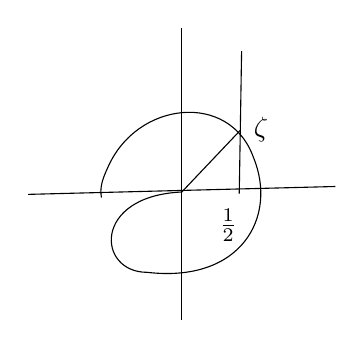
\begin{tikzpicture}[x=1cm,y=1cm]
\draw (-1.95,-.03)--(1.95,.07);
\draw (0,-1.62)--(0,2.08);
\draw (0,0) .. controls (-1.14,-.05) and (-1.08,-1.02) .. (-.44,-1.02) .. controls (.76,-1.16) and (1.22,-.31) .. (.91,.44) .. controls (.61,1.28) and (-.57,1.16) .. (-.94,.31) .. controls (-1.02,.14) and (-1.04,.04) .. (-1.02,-.07);
\draw (.73,-.02)--(.76,1.79);
\draw (0,0)--(.74,.78);
\node[right] at (.79,.79) {$\zeta$};
\node[below] at (.59,-.09) {$\frac12$};
\end{tikzpicture}}

\diagram{\begin{tikzcd}[ampersand replacement=\&,row sep=large,column sep=large]
\Pi_{0,3}^{\mathbb D'} \arrow[r] \arrow[d] \& \Pi_{0,3}^{\mathbb D}=\{\rho,\sigma\mid\rho^3=\sigma^2=1\} \arrow[d,Rightarrow] \\
\deleted{\unsure{\mathbb Z/4\mathbb Z}}\,\inserted{\unsure{\mathbb D'_3}} \arrow[r] \arrow[d] \arrow[ur,phantom,"\unsure{\mathrm{cart}}"{description}] \& \deleted{\unsure{\mathbb Z/2\mathbb Z}}\,\inserted{\unsure{\mathbb D_3}} \arrow[d] \\
\mathbb Z/4\mathbb Z \arrow[r,no head] \arrow[ur,phantom,"\unsure{\mathrm{cart}}"{description}] \& \mathbb Z/2\mathbb Z
\end{tikzcd}}

\margin{$\deleted{\rho\mapsto0,\quad\sigma\mapsto1}$\par
$\rho\mapsto0$\par
$\sigma\mapsto1$}

\margin{\unsure{On remonte} $\rho,\sigma$ en $\deleted{\unsure{\rho,\sigma}}\ \rho',\sigma'$\par
$\rho'=(\rho,2),\quad\sigma'=(\sigma,\deleted{\unsure{2}}\inserted{3})$\par
\unsure{on a}
$\rho'^{\,6}=\sigma'^{\,4}=1,$\par
$\rho'^{\,3}=\sigma'^{\,2}=(\underbrace{1,2\bmod4}_{\omega})$.}

\margin{On vérifie alors aisément que\par
$\mathrm S\ell(2,\mathbb Z)\simeq\{\rho',\sigma'\mid \unsure{\rho'^{\,6}=\sigma'^{\,4}=1},\ \unsure{\rho'^{\,3}=\sigma'^{\,2}}\}$.}

\margin{\figure{\begin{tikzpicture}[x=1cm,y=1cm]
\draw[->] (2.92,3.25) .. controls (2.82,2.34) and (1.35,2.38) .. (1.05,1.46) .. controls (.92,1.12) and (.86,.77) .. (.71,.58);
\draw (0.05,2.24) .. controls (.42,1.64) and (.29,1.03) .. (.21,.96) .. controls (.12,.88) and (.24,.73) .. (.35,.68);
\draw (.59,.98) .. controls (.43,.46) and (.48,.12) .. (.35,-.02) .. controls (.62,.12) and (.63,-.29) .. (.67,-.72);
\end{tikzpicture}}}

Ainsi $\Pi_{0,3}^{\mathbb D'}\simeq\mathrm S\ell(2,\mathbb Z)$ \unsure{apparaît} comme extension de $\Pi_{0,3}^{\mathbb D}$ par $\mathbb Z/2\mathbb Z$, image inverse \deleted{\unsure{de}} l'ext. \inserted{$\mathbb D'_3$} de $\mathbb D_3$ par $\mathbb Z/2\mathbb Z$, ou de l'ext. $\mathbb Z/4\mathbb Z$ de $\mathbb Z/2\mathbb Z$ par $\mathbb Z/2\mathbb Z$, via $\Pi_{0,3}^{\mathbb D}\to\mathbb D_3$ \unsure{resp.} composé $\Pi_{0,3}^{\mathbb D}\to\deleted{\unsure{\mathbb D_3}}\mathbb Z/2\mathbb Z$. \unsure{C'est} une ext. de $\mathbb D'_3$ par un \unsure{gr.} $\simeq\Pi_{0,3}$, \unsure{de base} $\rho_0,\rho_1,\rho_\infty$ \unsure{---}

\margin{15}

\scanpage{17}

\deleted{\diagram{\begin{tikzcd}[ampersand replacement=\&,column sep=small,row sep=large]
\& \vec S(\unsure{X_0|X_\bullet})\simeq G_0 \arrow[dl] \arrow[d] \arrow[dr] \& \\
S(X_0)\simeq G_0/H_S \& A(X_0)\simeq G_0/H_A, \& F(X_0)\simeq G_0/H_F
\end{tikzcd}}}

\deleted{\[
H_S\cap H_A=e,\qquad H_A\cap H_F=e,\qquad H_S\cap H_F=e
\]}

\deleted{\unsure{i.e.|i.a.}
\[
G_0\hookrightarrow G_0/H_S\times G_0/H_A,\qquad
G_0\hookrightarrow G_0/H_A\times G_0/H_F,\qquad
G_0\unsure{\hookrightarrow|\subset}\deleted{\unsure{G_0|H_S}}/H_A\times G_0/H_F
\]}

\deleted{\figure{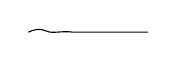
\begin{tikzpicture}[x=1cm,y=1cm]
\draw (0,0).. controls (.1,.04) and (.14,.05) .. (.24,.01).. controls (.31,-.02) and (.43,.02) .. (.57,0)--(1.52,0);
\end{tikzpicture}}}

\margin{\uline{\unsure{Cas non orienté}}}

\deleted{Considérons la catégorie des polyèdres (non orientés) de type donné; il y a des foncteurs}

\deleted{\[
\begin{array}{l}
S\\
\vec A\\
F\\
\deleted{\unsure{A|R}}
\end{array}
\]}

\deleted{\diagram{\(\begin{array}{lll}
A_1 & \text{relation d'incidence entre }S\text{ et }A & \text{(}\unsure{\text{arêtes orientées}}\text{ au sens }1\text{)}\\
A_2 & \rule{3.2cm}{0.25pt}\ A\text{ et }F & (\rule{2.8cm}{0.25pt}\ 2)\\
A_3 & \text{rel. d'incidence entre }\unsure{S|B}\text{ et }F &
\end{array}\)}}

\deleted{\[
R=\deleted{\unsure{A_3}}\unsure{\simeq|=}A_1\times_A A_2
\]
\deleted{\unsure{relation} d'incidence entre $S$ et $F$}
\inserted{\unsure{triplets ou drapeaux|triplets de drapeaux} $(s,a,f)$\quad$s\unsure{\leq|<}a<f$.}}

\deleted{\diagram{\begin{tikzcd}[ampersand replacement=\&,row sep=small,column sep=small]
\& R \arrow[dl] \arrow[d] \arrow[dr] \& \\
S\&A\&F
\end{tikzcd}}}

\deleted{\[
\begin{aligned}
A_1&=\operatorname{Im}(R\to S\times A)\\
A_2&=\operatorname{Im}(R\to A\times F)\\
A_3&=\operatorname{Im}(R\to S\times F)
\end{aligned}
\]}

\deleted{$\Omega$ ens des orientations}

\deleted{\[
{A_1}_{\Omega}\simeq\unsure{{A_2}_{\Omega}}\simeq{A_3}_{\Omega}\qquad(
\]}

\[
\mathrm{Pol}_{\unsure{\tau|t}}\qquad
\mathrm{Pol}_{\tau}^{\unsure{\mathrm{or}}}\simeq
\mathrm{Pol}_{\tau}\deleted{\unsure{/\Omega}}\inserted{{}_{/\Omega}}
\]

\margin{16}

\scanpage{18}
\mspage{6}

$S\mathcal T_{1,1}\simeq$ \unsure{image inverse} de $\mathrm S\ell(2,\mathbb Z)$ dans $\unsure{\deleted{\mathrm G\ell}\mathrm S\ell(2,\mathbb R)^{\sim}|\mathrm G\ell(2,\mathbb R)^{\sim}}$
\[
\simeq\{\rho,\sigma\mid\rho^3=\sigma^2\ (=\omega)\}
\]
\margin{\unsure{(}\unsure{élém\textsuperscript{t}|él\textsuperscript{mt}} central}

\[
\mathcal T_{11}=S\mathcal T_{11}/\langle\omega^2\rangle
\]

\[
\begin{array}{ll}
(\mathcal T_{11})_{\mathrm{ab}}\simeq\mathbb Z & (\mathcal T_{11})_{\mathrm{ab}}\simeq\mathbb Z/12\mathbb Z\\[4pt]
\deleted{(\rho,\sigma)} & \\
\rho\longmapsto2 & \rho\longmapsto2\bmod12\\
\sigma\longmapsto3 & \sigma\longmapsto3\bmod12\\
\omega\longmapsto\unsure{6|8} &
\end{array}
\]

\diagram{\begin{tikzcd}[ampersand replacement=\&,row sep=large,column sep=small,nodes in empty cells]
\& 1 \& \& 1 \\
\& \mathcal T_{11} \arrow[u] \arrow[r] \& \deleted{\unsure{\mathcal T_{\mathrm{ab}}}} \arrow[r] \& \mathbb Z/12\mathbb Z \arrow[u] \\
\unsure{\widetilde\omega|\bar\omega}=\omega^{2\deleted{\unsure{4}}} \& S\mathcal T_{11} \arrow[u] \arrow[rr] \arrow[ur,phantom,"\deleted{\text{cartésien}}"{description}] \& \& \mathbb Z \arrow[u] \\
\uline{1} \arrow[u] \& \mathbb Z \arrow[u] \arrow[rr,"\mathrm{id}"] \& \& \mathbb Z \arrow[u,"12"] \\
\& 1 \arrow[u] \& \& 1 \arrow[u]
\end{tikzcd}}

\margin{donc $S\mathcal T_{11}$ se déduit de $\mathcal T_{11}$ par image inverse de l'ext. canonique de $\mathbb Z/12\mathbb Z$ par $\mathbb Z$, via $\mathcal T_{11}\to\mathbb Z/12\mathbb Z$.}

\deleted{une normalisation de $(K,\unsure{K_0|N|k_0})$, \unsure{alors} elle est \unsure{spéciale} : la cat. des rev. étales dans $\unsure{K'_fN|K'_{fN}}$ -- \deleted{\illegible{1}} $\Delta$ \unsure{rev.|i.e.} $\Delta$ top. \unsure{a} une unique normalisation pour laquelle la projection \unsure{est|soit} un \unsure{morphisme} de $\Delta$-complexes \unsure{normalisés}. [Mais attention, \unsure{ça ne marche} \uline{\unsure{pas}} pour \unsure{strictes normalisations} \unsure{$\overline{\mathrm m}$|néc.}\ldots]}

\deleted{\unsure{8.|$\beta$.} \unsure{Groupes|Groupe} et groupoïdes \unsure{fondamentaux|fondamental}. On \unsure{montrera|montre} la relation entre construction top. et construction algébrique.}

\margin{17}

\scanpage{19}

% pencil numeral at the top right corner; no other foliation numeral is visible on this sheet
\margin{8v}

\figure{\scalebox{0.90}{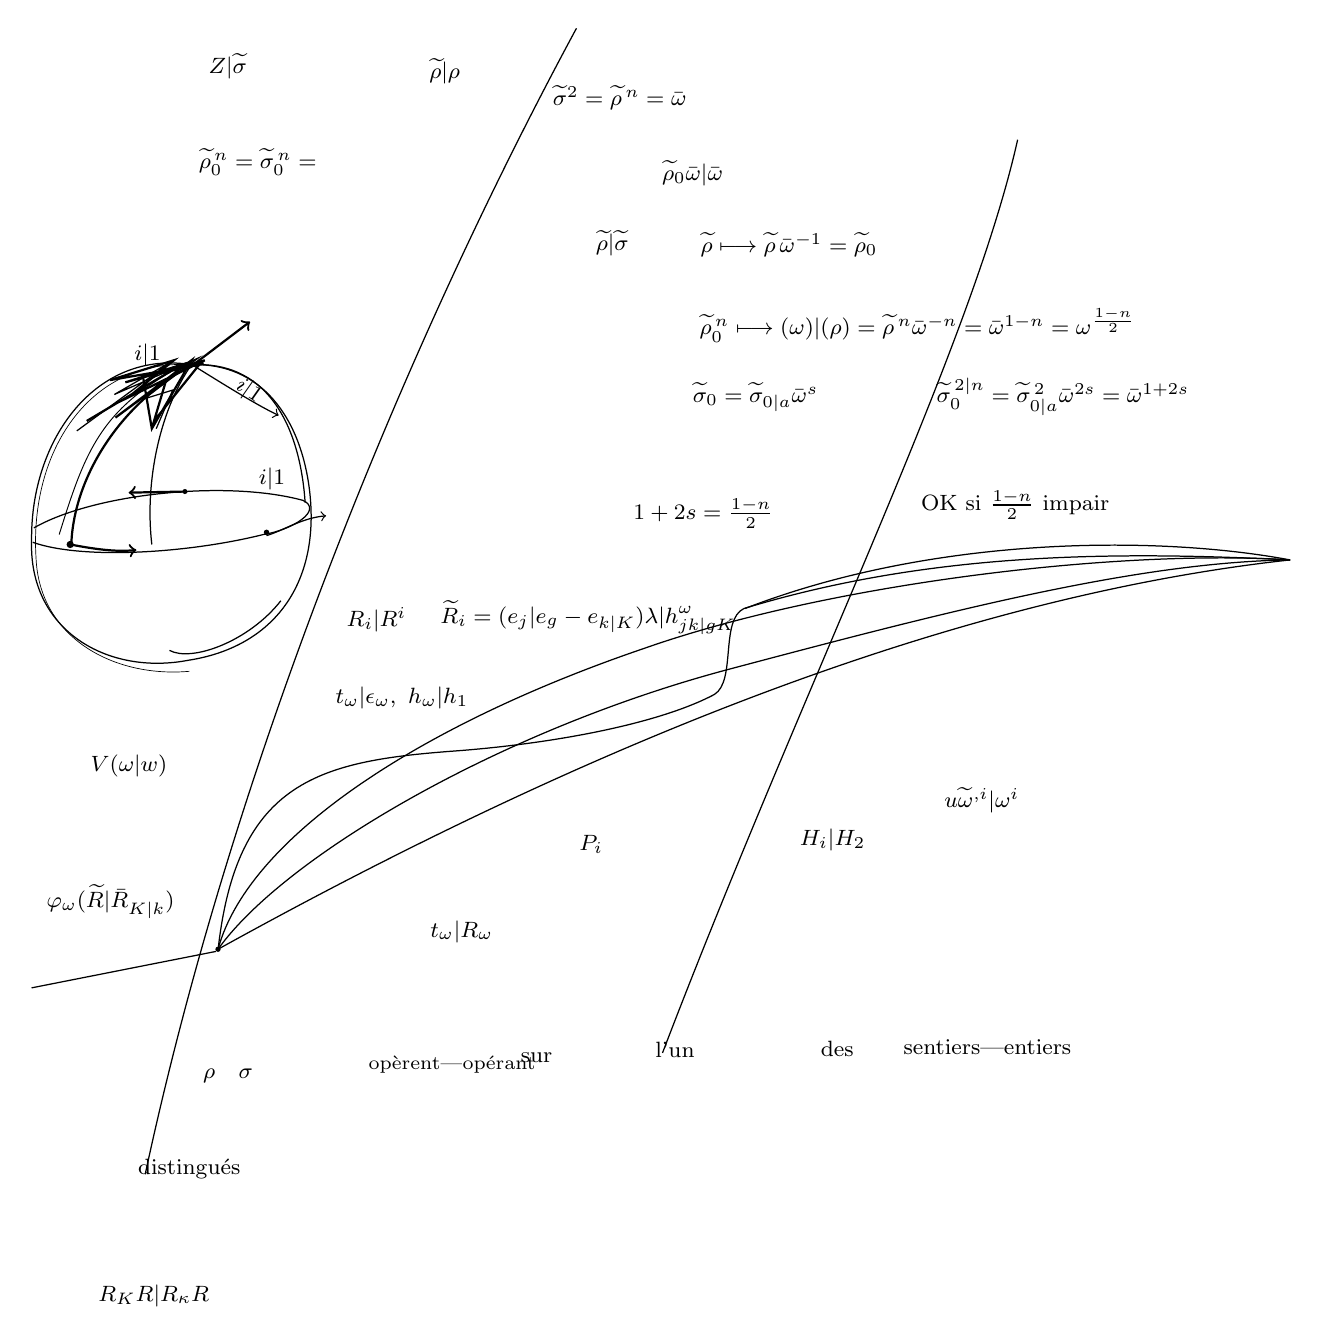
\begin{tikzpicture}[x=.014cm,y=-.014cm,every node/.style={font=\footnotesize,inner sep=0pt},line width=.45pt]
\node[anchor=west] at (385,80) {$\deleted{\unsure{\mathbb Z|\widetilde\sigma}}$};
\node[anchor=west] at (585,85) {$\deleted{\unsure{\widetilde\rho|\rho}}$};
\node[anchor=west] at (376,167) {$\widetilde\rho_0^{\,n}=\widetilde\sigma_0^{\,n}=$};
\node[anchor=west] at (697,109) {$\widetilde\sigma^2=\widetilde\rho^{\,n}=\bar\omega$};
\node[anchor=west] at (796,177) {$\deleted{\unsure{\widetilde\rho_0\bar\omega|\bar\omega}}$};
\node[anchor=west] at (736,241) {$\deleted{\unsure{\widetilde\rho|\widetilde\sigma}}$};
\node[anchor=west] at (831,242) {$\widetilde\rho\longmapsto\widetilde\rho\,\bar\omega^{-1}=\widetilde\rho_0$};
\node[anchor=west] at (830,315) {$\widetilde\rho_0^{\,n}\longmapsto\deleted{\unsure{(\omega)|(\rho)}}=\widetilde\rho^{\,n}\bar\omega^{-n}=\bar\omega^{1-n}=\omega^{\frac{1-n}{2}}$};
\node[anchor=west] at (824,380) {$\widetilde\sigma_0=\widetilde\sigma_{\unsure{0|a}}\bar\omega^s$};
\node[anchor=west] at (1045,380) {$\widetilde\sigma_0^{\,\unsure{2|n}}=\widetilde\sigma_{\unsure{0|a}}^{\,2}\bar\omega^{2s}=\bar\omega^{1+2s}$};
\node[anchor=west] at (770,486) {$1+2s=\frac{1-n}{2}$};
\node[anchor=west] at (1031,478) {OK si $\frac{1-n}{2}$ \uline{impair}};

\draw (328,1085) .. controls (405,726) and (557,346) .. (719,46);
\draw (797,975) .. controls (925,640) and (1077,335) .. (1119,147);

\draw (370,351) .. controls (284,337) and (224,418) .. (225,510) .. controls (222,592) and (294,633) .. (367,619) .. controls (445,607) and (487,549) .. (477,465) .. controls (469,399) and (433,349) .. (370,351);
\draw[line width=.25pt] (371,351) .. controls (277,345) and (223,430) .. (229,526) .. controls (232,599) and (300,635) .. (368,629);
\draw (350,610) .. controls (370,621) and (422,602) .. (451,565);
\draw (227,499) .. controls (281,468) and (401,455) .. (471,474) .. controls (490,483) and (461,501) .. (435,505) .. controls (367,522) and (271,528) .. (226,512);
\draw[line width=.8pt,->] (260,514) .. controls (281,518) and (301,521) .. (320,519);
\draw[line width=.8pt,->] (366,466)--(313,467);
\draw[->] (438,506) .. controls (454,501) and (470,490) .. (492,488);
\fill (260,514) circle[radius=3.3];
\fill (438,503) circle[radius=2.5];
\fill (364,466) circle[radius=2.3];
\draw (334,514) .. controls (327,454) and (343,389) .. (370,351);
\draw[line width=.8pt] (261,514) .. controls (263,455) and (303,388) .. (370,351);
\draw[line width=.35pt] (250,505) .. controls (274,428) and (288,390) .. (365,350);
\draw[line width=.8pt,->] (369,353)--(423,312);
\draw[->] (372,352) .. controls (398,368) and (428,387) .. (449,397);
\draw (377,351) .. controls (437,351) and (468,403) .. (473,476);
\node at (330,342) {$\unsure{i|1}$};
\node[rotate=-35] at (422,375) {$\unsure{i|1}$};
\node at (443,455) {$\unsure{i|1}$};
\draw[line width=.8pt] (275,402)--(361,351)--(310,367)--(382,347)--(312,381)--(354,347)--(296,365)--(377,351)--(336,402)--(347,365)--(301,399)--(370,347)--(334,409)--(326,362)--(381,350);
\draw (266,411)--(352,348)--(300,378)--(376,345)--(327,382)--(353,374)--(338,409);

\node[anchor=west] at (510,582) {$\unsure{R_i|R^i}$};
\node[anchor=west] at (595,580) {$\widetilde R_{\unsure{i}}=(\unsure{e_j|e_g}-e_{\unsure{k|K}})\unsure{\lambda|h}^{\omega}_{\unsure{jk|gK}}$};
\node[anchor=west] at (500,653) {$\unsure{t_\omega|\epsilon_\omega},\ \unsure{h_\omega|h_1}$};
\node[anchor=west] at (278,715) {$V(\unsure{\omega|w})$};
\node[anchor=west] at (238,838) {$\varphi_\omega(\unsure{\widetilde R|\bar R}_{\unsure{K|k}})$};
\node[anchor=west] at (721,786) {$P_i$};
\node[anchor=west] at (586,865) {$\deleted{\unsure{t_\omega|R_\omega}}$};
\node[anchor=west] at (921,782) {$\deleted{\unsure{H_i|H_2}}$};
\node[anchor=west] at (1052,746) {$u\unsure{\widetilde\omega^{,i}|\omega^i}$};

\draw (225,916)--(392,883);
\fill (394,881) circle[radius=2.4];
\draw (394,882) .. controls (411,727) and (487,710) .. (612,701) .. controls (702,694) and (795,676) .. (844,650) .. controls (864,638) and (849,582) .. (871,572) .. controls (1039,521) and (1205,520) .. (1366,528);
\draw (394,881) .. controls (422,778) and (581,676) .. (781,608) .. controls (949,549) and (1211,518) .. (1366,528);
\draw (394,881) .. controls (454,797) and (649,683) .. (854,628) .. controls (1057,574) and (1228,530) .. (1366,528);
\draw (394,881) .. controls (721,700) and (1056,562) .. (1366,528);
\draw (872,572) .. controls (1045,505) and (1249,506) .. (1366,528);

\node[anchor=west] at (380,996) {$\rho\quad\sigma$};
\node[anchor=west,font=\scriptsize] at (530,986) {\unsure{opèrent|opérant}};
\node[anchor=west] at (668,979) {sur};
\node[anchor=west] at (790,972) {l'un};
\node[anchor=west] at (940,971) {des};
\node[anchor=west] at (1015,970) {\unsure{sentiers|entiers}};
\node[anchor=west] at (321,1080) {distingués};
\node[anchor=west] at (285,1195) {$\deleted{\unsure{R_KR|R_\kappa R}}$};
\end{tikzpicture}}}
